%%%%%%%%%%%%%%%%%%%%%%%%%%%%%%%%%%%%%%%%%
% University/School Laboratory Report
% LaTeX Template
% Version 3.1 (25/3/14)
%
% This template has been downloaded from:
% http://www.LaTeXTemplates.com
%
% Original author:
% Linux and Unix Users Group at Virginia Tech Wiki 
% (https://vtluug.org/wiki/Example_LaTeX_chem_lab_report)
%
% License:
% CC BY-NC-SA 3.0 (http://creativecommons.org/licenses/by-nc-sa/3.0/)
%
%%%%%%%%%%%%%%%%%%%%%%%%%%%%%%%%%%%%%%%%%

%----------------------------------------------------------------------------------------
%	PACKAGES AND DOCUMENT CONFIGURATIONS
%----------------------------------------------------------------------------------------

\documentclass{article}

\usepackage[version=3]{mhchem} % Package for chemical equation typesetting
\usepackage{siunitx} % Provides the \SI{}{} and \si{} command for typesetting SI units
\usepackage{graphicx} % Required for the inclusion of images
\usepackage{natbib} % Required to change bibliography style to APA
\usepackage{amsmath} % Required for some math elements 
\usepackage[colorlinks = true,
            linkcolor = blue,
            urlcolor  = blue,
            citecolor = blue,
            anchorcolor = blue]{hyperref}
\setlength\parindent{0pt} % Removes all indentation from paragraphs

\newcommand{\horrule}[1]{\rule{\linewidth}{#1}} % Create horizontal rule command with 1 argument of height

\renewcommand{\labelenumi}{\alph{enumi}.} % Make numbering in the enumerate environment by letter rather than number (e.g. section 6)

%\usepackage{times} % Uncomment to use the Times New Roman font

%----------------------------------------------------------------------------------------
%	DOCUMENT INFORMATION
%----------------------------------------------------------------------------------------

%\title{
%	\horrule{0.5pt} \\[0.4cm] % Thin top horizontal rule
%	\huge A Parametrizable CPU Cache in System Verilog  \\ with  Approximate LRU Page Replacement Policy
%	\horrule{2pt} \\[0.5cm] % Thick bottom horizontal rule
%\normalfont \normalsize 
%\textsc{ECE 485} \\ 
%
%}
\title{	
%\normalfont \normalsize 
%\textsc{ECE 485} \\ [25pt] % Your university, school and/or department name(s)
%\horrule{0.5pt} \\[0.4cm] % Thin top horizontal rule
\LARGE A Parametrizable CPU Cache in System Verilog \\
\large with Approximate LRU Page Replacement Policy 
\horrule{0.5pt} \\[0.5cm] % Thick bottom horizontal rule
}

\author{Matthew Whiteside \& Jared Rue} % Author name

\date{\normalsize\today} % Today's date or a custom date


\begin{document}

\maketitle % Insert the title, author and date


% If you wish to include an abstract, uncomment the lines below
% \begin{abstract}
% Abstract text
% \end{abstract}

%----------------------------------------------------------------------------------------
%	SECTION 1
%----------------------------------------------------------------------------------------

\section{Overview}

We've implemented a CPU cache with the following features: 
\begin{itemize}
	\item Parametrizable:
		\begin{itemize}
			\item word size (1 byte by default)
			\item page size (a.k.a. words per page)
			\item number of rows (a.k.a. pages; 16 by default)
			\item number of sets (a.k.a. associativity)
			\item address bus width (16 bits by default)
		\end{itemize}
	\item A pseudo-LRU page replacement which implements the `clock' algorithm (detailed in section 2 below)
	\item Some (unrealistic) \textbf{simplifying assumptions} of the design:
		\begin{itemize}
			\item the bus to main memory is the width of a full page (8 bytes/64 bits by default), which means an entire cache line (page) is filled in one cycle when the fetch returns from DRAM
			\item Changing operations while one is in progress is not really handled robustly.  In other words if you change from a read to a write operation before the read is finished, the behavior is undefined.  This means you must hold the current operation until you receive the hit signal
		\end{itemize}
%	\item Some of the more sophisticated features of a more robust cache which we did not implement:
%		\begin{itemize}
%			\item Prioritizing reads over writes
%			\item write buffering
%		\end{itemize}

\end{itemize}  


\section{Page Replacement Policy}
As stated above we've implemented the clock algorithm.  It works in the following way.  Each set has 3 extra bits per row, a valid bit, a used bit, and a dirty bit.  At any time, the LRU\_set\_ptr is pointing at one of the sets.  If the cache receives a request, the first thing checked is whether the address results in a hit.  For a cache hit there's no need to replace anything.  Otherwise (on a cache miss), if the used bit is set in the LRU\_set, we first clear it, then increment the LRU\_set\_ptr.  During the next cycle, we check the used bit in the new LRU\_set.  If it's used, we clear it and increment the LRU\_set\_ptr again.  This process continues until we've either found a set whose used bit is clear, or arrived back at the original set, whose used bit we cleared earlier, and is now available.\\ 

This reason we chose this algorithm is that it is relatively simple, and performs well compared to a true LRU algorithm (see page 12 of [1]).

\section{Operation} Reading/writing is controlled by the `we\_L' signal, i.e., active-low write enable.  When we\_L is high, a read will be performed. A new address can be applied after the hit signal goes high. 

\section{State Transition Diagram}
\begin{figure}[h]
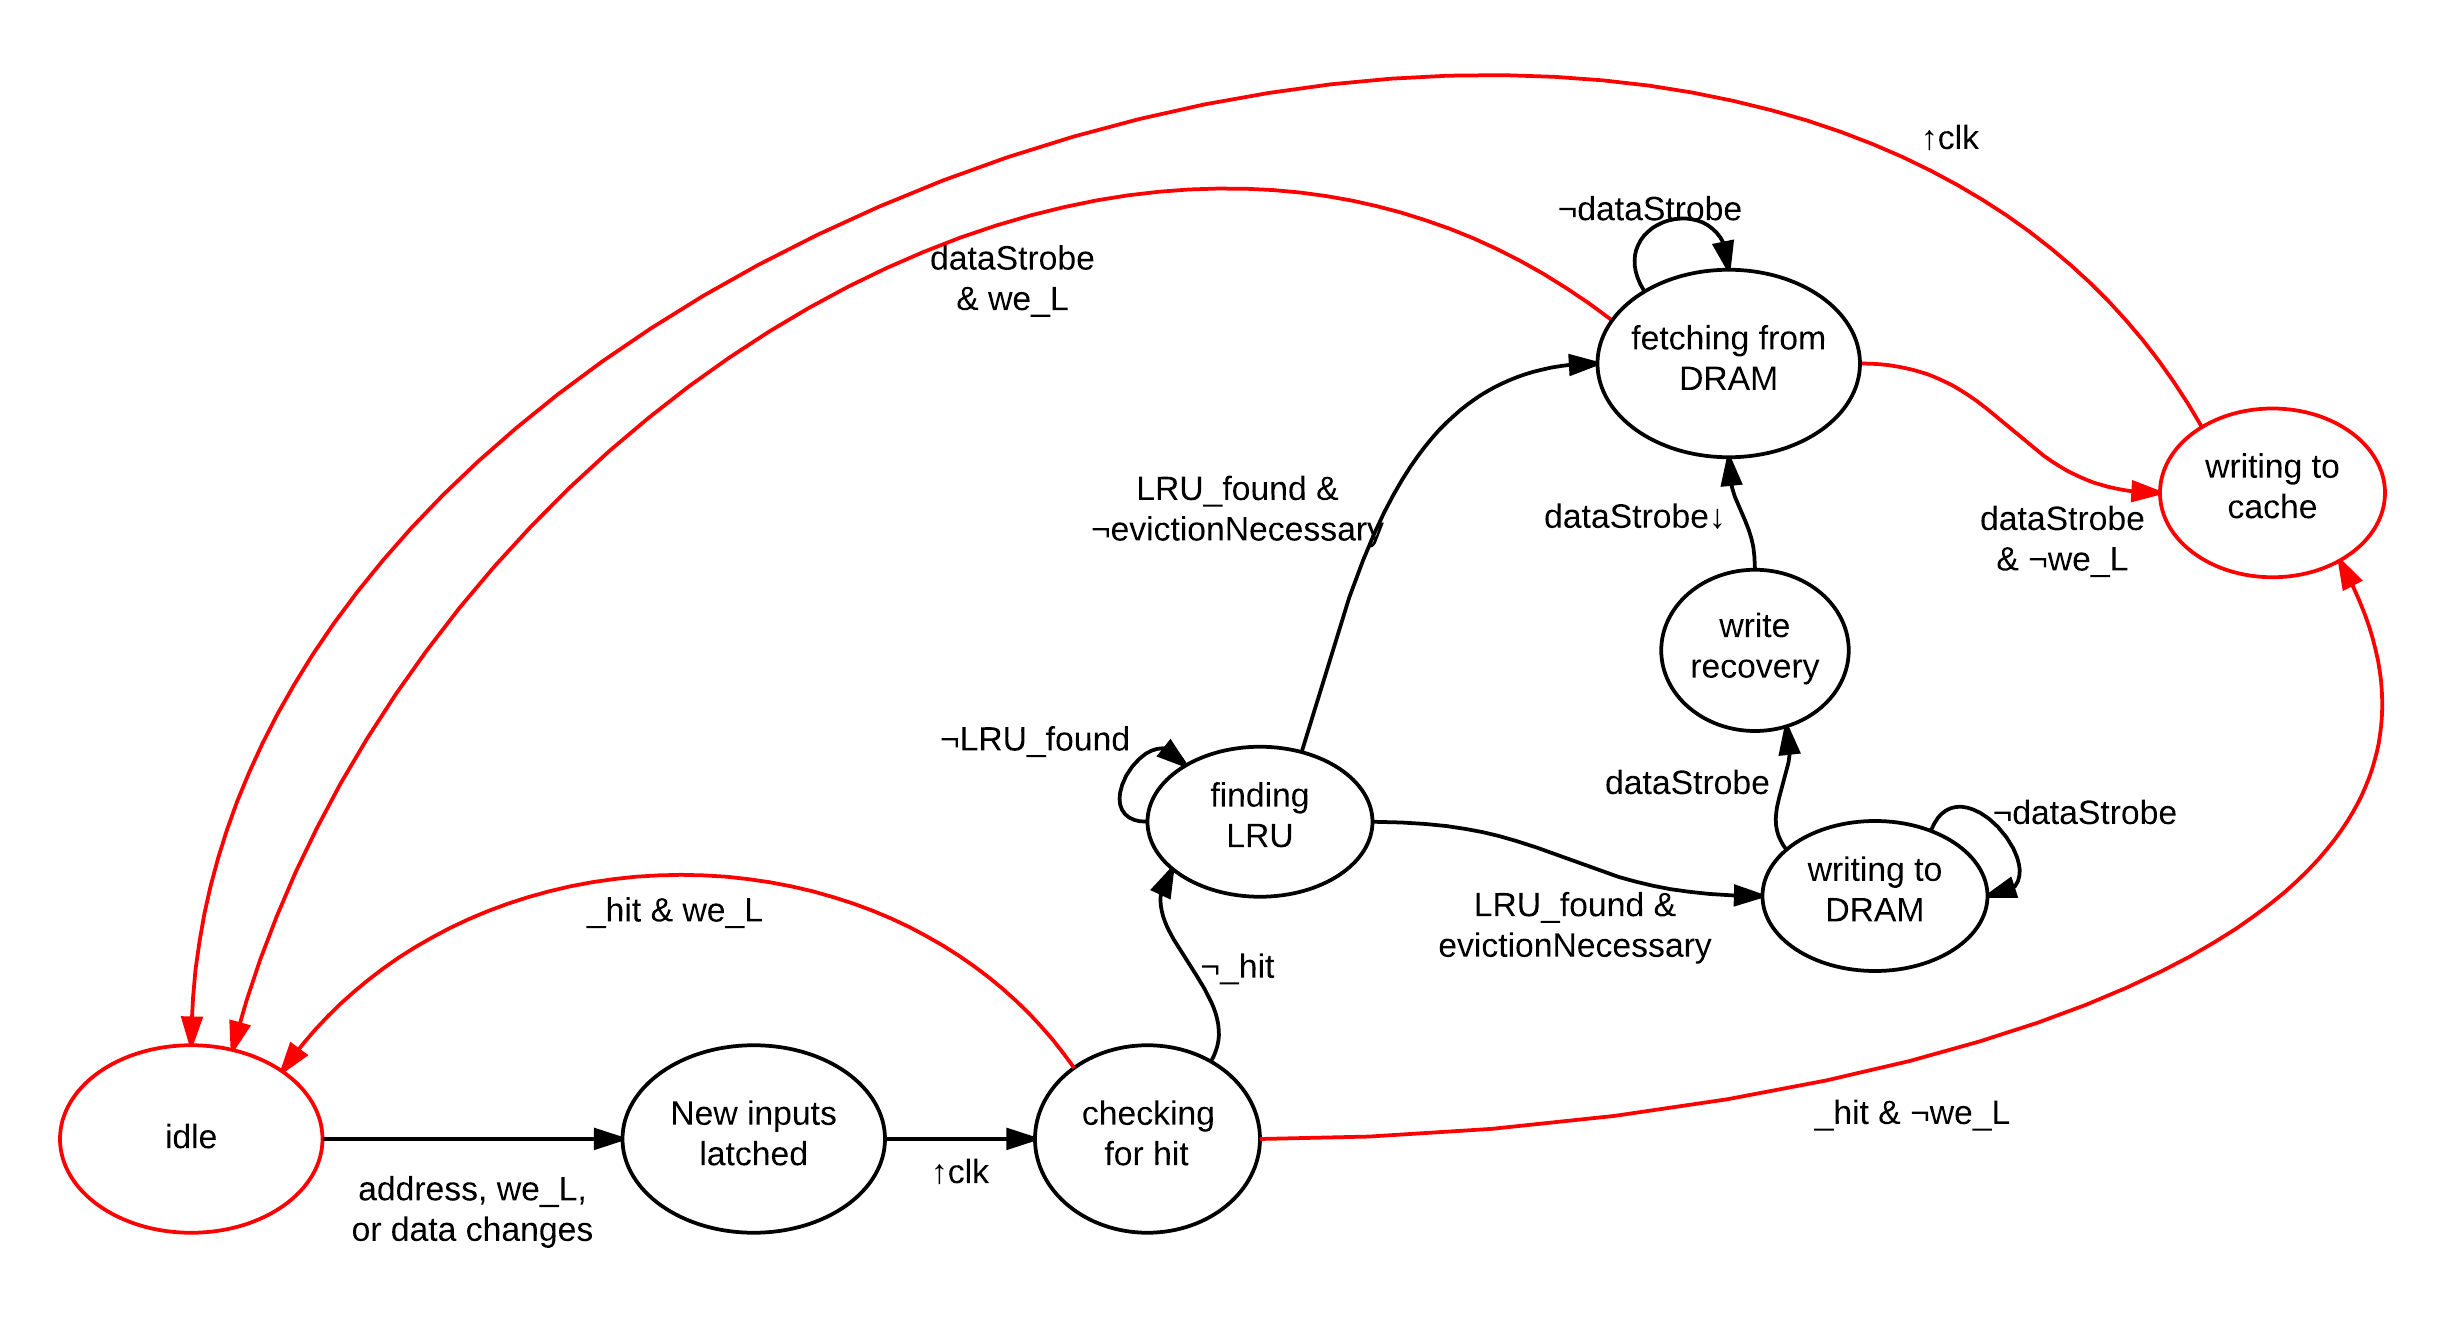
\includegraphics[scale=0.6]{state-diagram.png}

\caption{Red arcs indicate the internal `\_hit' signal goes high, and then the red state bubbles that follow are when the external `hit' signal goes high.}
\centering
\end{figure}

\section{Test Cases}
We tested the following 6 scenarios:
\begin{enumerate}
	\item[1.] Read $A_{1}$/write $A_{2}$/read $A_{1}$: and expect that the second read to $A_{1}$ results in a cache hit, and does not result in a latency of many cycles.  Also see attached timing diagram for this scenario.
	\item[2.] Successive reads that map to the same row index should go to different sets.
	\item[3.] sequential writes should go to the same set \& cache line, and not cause cache misses
	\item[4.] Reads to occupied sets/lines should result in evictions.
	\item[5.] Data should be available on the outputs 3 cycles after the hit signal is received.
	\item[6.] When the machine enters the FINDING\_LRU state, and all the sets in the specified row are full, it should transition to WRITING\_TO\_DRAM between 2 and 5 cycles later.
\end{enumerate}
\section{References} 
\begin{enumerate}
	\item[1.] Arpaci-Dusseau, 2014.  \href{http://pages.cs.wisc.edu/~remzi/OSTEP/vm-beyondphys-policy.pdf}{Three Easy Pieces}
\end{enumerate}





\end{document}